\documentclass[11pt]{article}

\usepackage{fullpage}
\usepackage[utf8]{inputenc}
\usepackage{color}
\usepackage{ragged2e}
\usepackage{parskip}
\usepackage[english]{babel}
\usepackage{float}  
\usepackage{caption}
\usepackage{graphicx}
\usepackage{subfig}

\begin{document}

\title{Final Report for Assembler and Extension - Digital Receipt System}
\author{Group 17 : Wei Yi Tee, Soon Zhi Ho (Brandon), Zirun Zhai, Ivy Tam}

\maketitle

\section{Assembler Structure}

We decided to split the \textbf{assembler} into these main files :

\begin{itemize}
	\item \textcolor{blue}{\textbf{\emph{assemble\_types.h}}}: Contains additional definitions of the types used throughout our assembler, eg:
	\begin{itemize}
	    \item struct {\textbf{instr\_str\_t}} which holds the mnemonic, original instruction string, an array of pointers to the start of each operand in the string and the assemble function pointer assigned during tokenizing.
	    \item {\textbf{program\_t}} is a list where the element either contains a {\textbf{instr\_str\_t}} to be assembled or a binary value (implemented as a union) and the address of the element in the program, mimicking byte addressing. 
	\end{itemize}
	\item \textcolor{blue}{\textbf{\emph{assemble.h}}}: Contains declarations of functions used in the main function of assemble these include - {\textbf{first\_pass}}, {\textbf{tokenizer}}, {\textbf{assemble\_instructions}} and {\textbf{binary\_writer}}.
	\item \textcolor{blue}{\textbf{\emph{assemble.c}}}: Contains the main function of the assembler. It calls functions declared in assemble.h where the implementations are distributed into relevant files.
	\begin{itemize}
	    \item The function {\textbf{first\_pass}} in {\textbf{assemble\_utils.c}} loads each line from an input assembly file to populate two linked lists - a symbol table mapping and a list of instruction strings
	    \item The function {\textbf{tokenizer}} in {\textbf{tokenizer.c}} splits the instruction strings into operands and assigns the correct mnemonic and assemble function pointer
	    \item The function {\textbf{assemble\_instructions}} assembles all tokenized instructions into binary by calling the appropriate assemble function for each instruction as assigned by the tokenizer. These functions are implemented in {\textbf{assemble\_instructions.c}}.
	    \item The function {\textbf{binary\_writer}} in {\textbf{assemble\_utils.c}} writes assembled binary code in little endian to a output binary file.	
	\end{itemize}
	\item\textcolor{blue}{\textbf{\emph{assemble\_instruction\_utils.h/c}}}: Contains other helper functions involved in assembling e.g. for parsing strings of different syntax to their correct binary encoding
	\item \textcolor{blue}{\textbf{\emph{symbol\_table\_utils.c/program\_utils.c.c}}}: Contains helper functions for manipulating the relevant list type and its elements
\end{itemize}
\section{Extension}
\subsection{Motivation and Use Of Extension}
Paper receipts are an unexpectedly large source of pollution. The production of paper receipts emits 4 billion pounds of CO2, uses approximately 13.2 billion gallons of water and 12.4 million trees every year just in America \cite{receiptStat}. Our group has decided to create a digital receipt system as an extension that would allow businesses to eliminate the need for paper receipts. This would mitigate the negative impact that paper receipts have on the environment. Moreover, digital receipts will allow for completely contactless payments, making social distancing due to the ongoing pandemic easier. These would allow our world to recover and improve. 

For example, a restaurant could utilise our extension so that the cashier generates receipts for its customers according to their meals. Editable orders allow the cashier to amend any careless mistakes made in a hurry or add orders, e.g. if a customer decides to have dessert. 
\subsection{Design Details Of Extension}
\begin{figure}[h]
\centering
    \subfloat[Flow Chart Of Initial Design]{{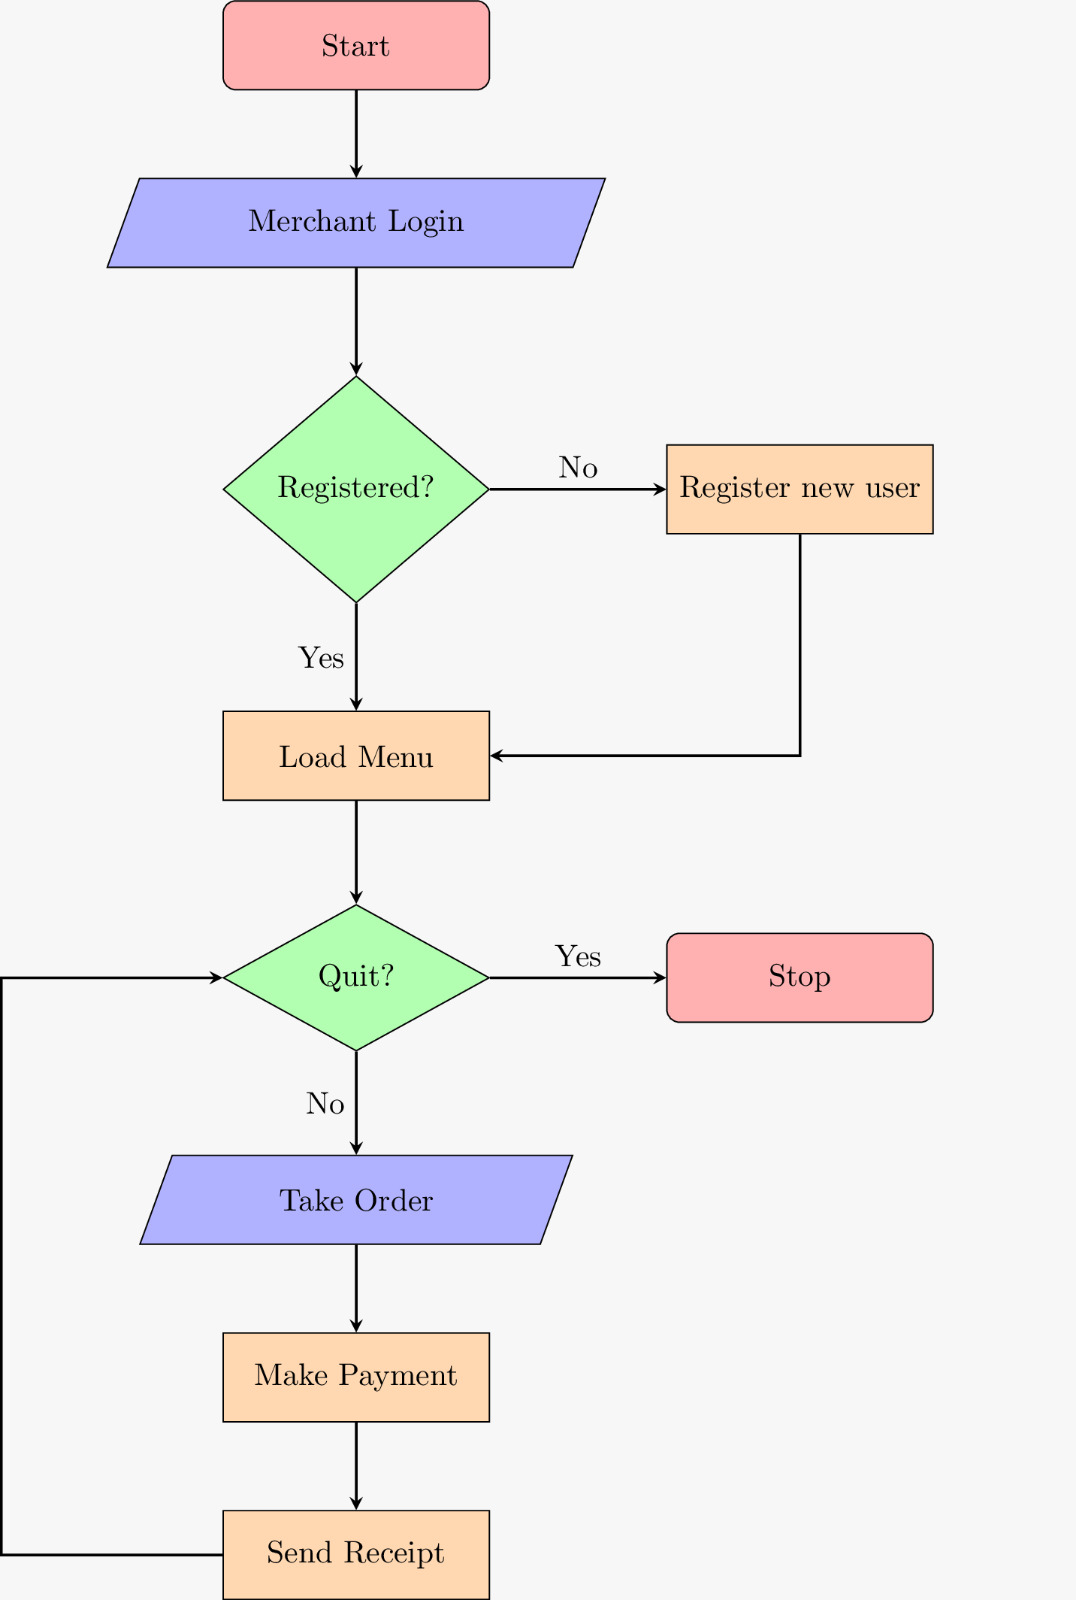
\includegraphics[height=8.75cm]{intial_design.jpeg} }}%
    \qquad
    \subfloat[Flow Chart of Final Design]{{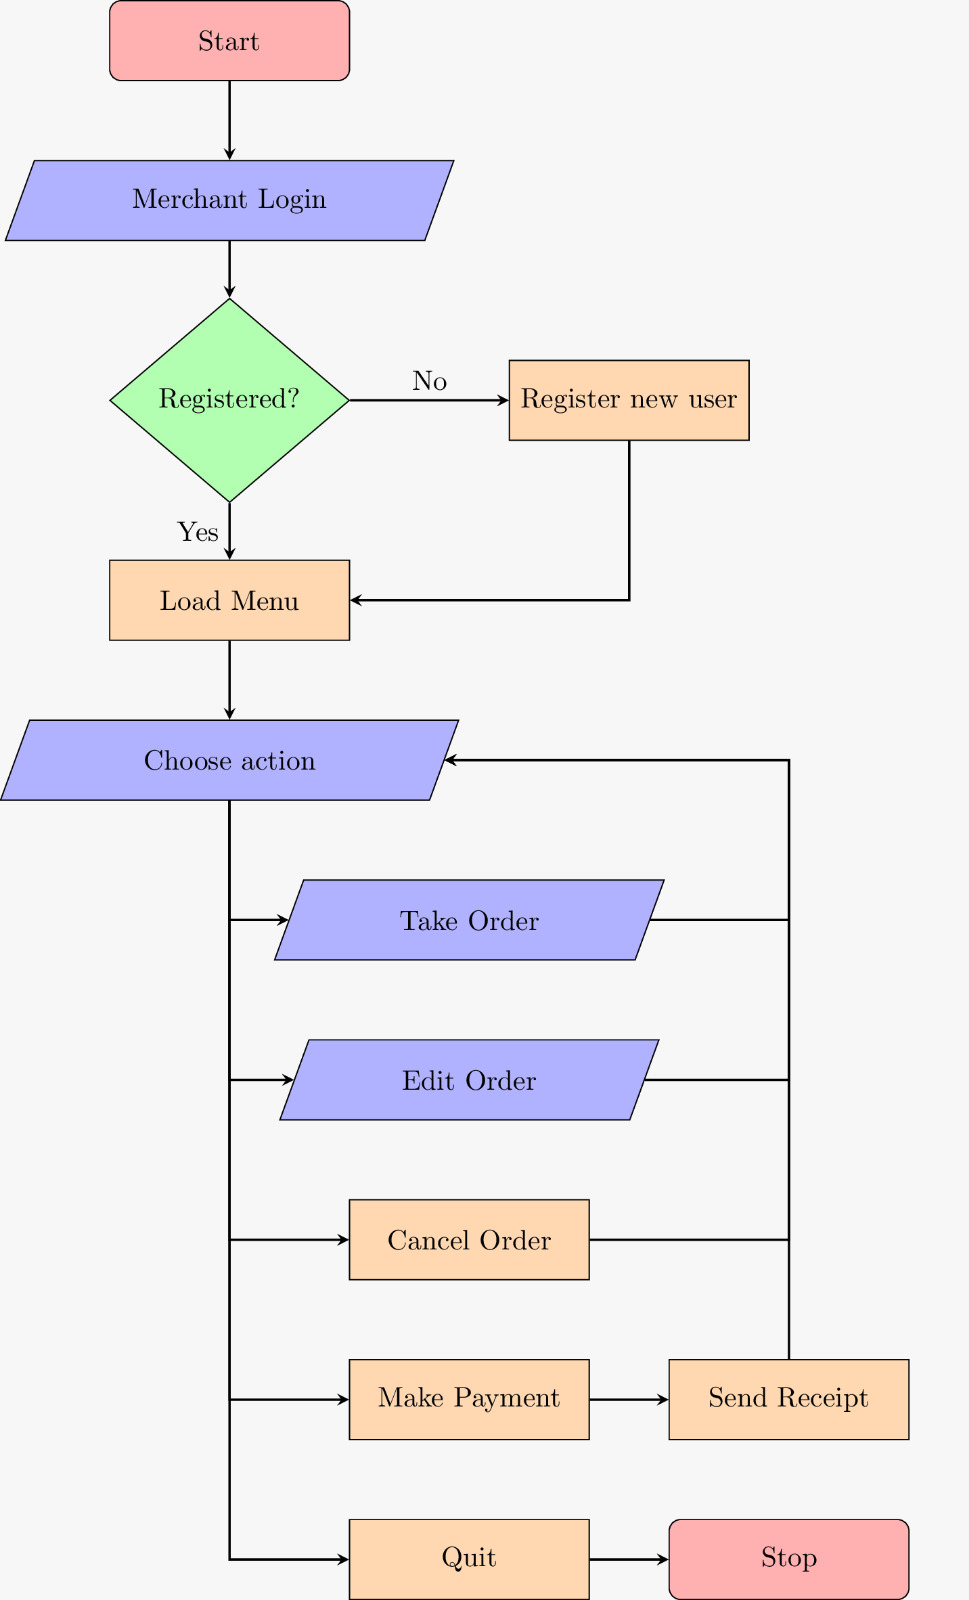
\includegraphics[height=8.75cm]{final_design.jpeg} }}%
    \caption{The final design was adapted to also suit businesses which have a pay later procedure (e.g. for restaurants) and allow for orders to be edited and cancelled.}%
    \label{fig:example}%
\end{figure}
The finalised design (Figure 1b) of our extension - a digital receipt system, first involves a login prompt for a merchant. The merchant enters an ID checked against existing merchant IDs. If the ID is found, the merchant will be prompted for their password. If the ID is not found, the merchant will be prompted for registration. Registering involves providing a password and a text file containing a menu of items. A folder corresponding to the merchant will be created which will store the menu and receipts issued by the merchant. 

After successfully logging in, the email address and password of the merchant will be requested so that the system will be able to send receipts to customers after it has been authenticated. The merchant’s menu will be automatically retrieved and loaded. 

Once the merchant’s data has been initialised, he/she can choose to carry out an action from a list, as shown below.

\textbf{0) Quits the program}

\textbf{1) Take order:}  
A new empty order is created and the menu is printed to display the list of items on sale. The merchant is responsible for adding items by specifying the item’s ID and quantity. After finalising the order, the merchant can either choose to have the order paid immediately or store it in a list of unpaid orders to pay later. Paying immediately prompts the merchant for a payment method and follows with the same principle as 4).

\textbf{2) Edit order:} 
An unpaid order is retrieved by entering the number corresponding to the customer name which can then be edited, and when finalised has the same options for payment as take order. 

\textbf{3) Cancel order:}
Using the same principle of retrieving for 2), an unpaid order can be removed. 

\textbf{4) Pay order: }
Using the same principle of retrieving for 2), an unpaid order will be made into a receipt containing the order and the total price to pay. The merchant is then prompted for a payment type which will be recorded in the receipt. It will be stored in the merchant’s folder uniquely identified by the current time. The customer’s email address will be requested to which the receipt will then be sent.
\subsection{Challenges in Extension Implementation}
As in the initial design (Figure 1a), our program initially had a more sequential control flow which limited the choice of operations that can be done by the user. We decided to introduce a switch statement for actions and a list for storing orders.

Upon attempting to implement an automatic test suite, we realized that our functions needed to be able to interact with text files for comparison against expected behaviour. Hence, we had to modify functions involving I/O operations to be able to read from and write to both the standard I/O streams as well as text files.

We came up with the idea of emailing receipts to customers for their personal reference. After a bit of research, we realised that we needed to connect to a Simple Mail Transfer Protocol (SMTP) server to be able to send emails. We tried creating our own network sockets in C, but weren’t able to initiate an encrypted session. Therefore, we decided to make use of the Python SMTPlib to write a short script for user authentication and sending emails. We then execute it from our main C program by the \emph{system()} function. 

For security considerations, we stored the passwords of registered users as hashes. Although peppers \cite{pepperStat} are controversial in industrial practice due to the lack of a mechanism to rotate keys, we decided to attempt an implementation of a random pepper appended to the end of each user input password before hashing with the djb2 function which is both computed efficiently and distributed well. However, this meant that we had to use brute force to identify the pepper when authenticating passwords. 


\subsection{Extension Testing}

We have conducted both manual and automatic testing to verify the functionality of our implementation.

We had a file {\textbf{runtest.c}} which ran automatic tests for some of our utility functions. We also manually ran our program with numerous variations in menu and orders to check that it worked as intended. To speed up testing, we also made text files which would simulate user input and passed it as an argument into our main program.

These methods have proven to be greatly effective, as they have helped us to discover and debug several errors in our implementation. 
For example, while running the program manually, we discovered that we initially freed up memory too early after editing an unpaid order and this resulted in a segmentation fault when the merchant tries to close the transaction. Additionally, our implementation previously had difficulties pinging the email server while operating on Mac OS due to permission issues with Python. 

One error that our test suite revealed was that our pepper function initially changed the last character of the user input password instead of appending a random character to the end of it. It was a lot more time-efficient than manual testing, especially when we had to test our code repeatedly while editing. However, we were unable to test registering using a text file as it involved prompting the user to move a menu.txt file. 



\section{Group Reflection}
Our teamwork improved after gaining experience from making the emulator. Instead of deciding on a rough implementation and refining after as we did with the emulator, we were more organised and discussed all aspects of our assembler’s structure before coding. We also made a document to outline the overall structure of our assembler where we noted each function and data type needed to be implemented. This allowed us to distribute the work more evenly and everyone was clear on the project's progress and direction. In future, we would continue to plan out our projects thoroughly before starting work to prevent confusion down the line.

We have effectively and efficiently communicated using Whatsapp, keeping each other updated on tasks we are working on or have completed. This platform may not work well for a different group dynamic if members do not use Whatsapp, or do not check their messages as often. In future, we would continue to choose a platform for communication that all members are willing to actively utilize.

 An obstacle we faced was that we were all new to using version control as a team. Nevertheless, we have adapted well and this challenge did not affect our progress greatly. Developing the habit of implementing many of our functions in separate files meant we had less git conflicts.  We did face problems with our git commits where a member’s commits would override another’s. However, we were able to quickly identify and revert the changes. Our experiences during this project would allow us to use version control more smoothly in future. 

\section{Individual Reflections}
\subsection*{\underline{Ivy Tam}}
 From this project, I feel that I have gained an insight on programming in a team by discovering the difficulties as well as benefits of group programming. One of the difficulties I initially faced was reusing and understanding code written by others to complete my tasks. However, my teammates were very helpful and willing to clarify their code. As we progressed through the project, I found it much easier to understand my teammates’ code as we developed the habit of commenting and programming in a consistent manner. Moreover I found it very interesting to see different methods and approaches implemented by my peers to the same problem.

I believe I fitted well in this group as I found it easy to communicate with my members and managed to work independently on code that we distributed fairly across the group. Furthermore, I enjoyed the synergy of our group, as we had insightful discussions of our overall designs and I was able to see how individual contributions came together as a working solution at a much faster pace than I am used to. I also enjoyed acquiring new skills such as latex and git with them as we were able to teach each other as we learnt. Overall, this project was a very challenging and rewarding experience.

\subsection*{\underline{Zhai Zirun}}
Through completing this project, I have gained valuable experience and insights on programming in a group, and have learned more about my own strengths and weaknesses.
Initially, I expected to have trouble understanding others’ code, and for my groupmates to understand mine. Indeed, there were instances where we had to clarify certain parts of the implementation with each other. However, I realized that one of my strengths was that I was able to comment and reorganize code to maximize clarity, reducing the frequency of such instances. Writing cleaner code had the additional benefit of making the process of debugging and restructuring my own code far easier. As such, I will keep up these habits in future when working both in a group and alone. Another of my strengths is my ability to present information clearly and precisely, allowing me to contribute greatly to the reports and presentation. 

One weakness of mine would be my unfamiliarity with git. I can recall several occasions where I wasted a good half hour figuring out how to merge my code safely, and I have accidentally overwritten group mates’ code before, which led to some confusion. However, after these experiences, I have learned how to use git more effectively, and I aim to apply it to future group projects.
I believe that I have fit quite well with this group. We have communicated effectively, and our differing thought processes have given rise to great ideas and heightened efficiency. In sum, I have enjoyed this experience greatly, and am eager for my next group programming project. 

\subsection*{\underline{Ho Soon Zhi (Brandon)}}
I came to university without much experience in programming and thought to myself that by the end of my course, I want to be able to build software that can improve our daily lives. About 10 months have passed since, my first year has been far from easy. I found most of the modules really abstract and had a hard time understanding the concepts. However, the group project has definitely boosted my morale, especially after finishing the extension. My biggest takeaway is that with the right team, I already possess the necessary skills to develop something useful.

Before starting the group project, I thought that my code style was quite readable. However, I immediately realised how much I depended on the auto-formatting function when coding in Java. Therefore, I forced myself to stick to a code editor and not use any IDEs in hopes of practicing good habits. I suppose it did help as my group mates complained much less about my code towards the end of the project. 

I do believe that I fit in with the group and that we complemented each other well. They were very responsible and would always look to see if we can split the work up in order to be as efficient as possible. Not only did we support and help each other out a lot, we also had loads of joking around, though I must say that all 4 of us really do need to learn to use Git properly!

\subsection*{\underline{Wei Yi Tee}}
Through this project, at the least, I strengthened my programming skills  and other technical skills including using Git and Valgrind. However, I found the worth of this project to be the new experience of group programming and designing for a project which is the largest I have done so far. 

I am very happy with my group and feel that we complement each other well. Our group emphasizes on communication, which I realise was crucial to our success. The amount of communication we had meant everyone was contributing their ideas and discussing for the best design and the most efficient workflow. A second factor which I think was important was the habit to plan out the program's structure thoroughly before starting to code. It helped to distribute jobs more evenly, reduce code redundancy between members and prevented the need to make major changes. The ARM11 parts went by smoothly but I felt that we were slightly messy in the extension due to time constraints and the absence of a concrete specification which could have been overcome with more detailed planning. In future projects, I will definitely enforce the above mentioned factors to improve workflow.

Being particular about code proved to be a strength and weakness. My code was more well-commented and of neater design, therefore being fairly easy to read. On the other hand, it consumed more time when I could have done more important and useful jobs especially under the time constraint we had. This is something I have to learn to balance Also, another weakness I will work on is coming up with appropriate git commit messages to increase readability. Overall, I have learnt a lot from this project and would like to conclude with a thanks to all my group members who have made this experience all the more fun and rewarding. 
\newpage

\begin{thebibliography}{9}
\bibitem{receiptStat} 
SAP BrandVoice: The Business Case For Eliminating Paper Receipts
\\\texttt{https://www.forbes.com/sites/sap/2019/12/16/eliminating-paper-receipts/\#3ee4431e5b97}
\bibitem{pepperStat}
NordPass: Password Peppering
\\\texttt{https://nordpass.com/blog/pepper-password/}
\end{thebibliography}



\break
\end{document}

